\documentclass[a4paper,12pt]{article}
\usepackage[T2A]{fontenc}  %поддержка кириллицы в ЛаТеХ
\addtolength{\hoffset}{-1.7mm} % горизонтальное смещение всего текста как целого
\usepackage[utf8]{inputenc}  %По умолчанию кодировка KOI8 для *nix-систем
\usepackage[english,russian]{babel} %определение языков в документе
\usepackage{amssymb,amsmath,amsfonts,latexsym,mathtext} %расширенные наборы
  % математических символов
\usepackage{cite}  %"умные" библиографические ссылки
%(сортировка и сжатие)
\usepackage{indentfirst} %делать отступ в начале параграфа
\usepackage{enumerate}  %создание и автоматическая нумерация списков
\usepackage{tabularx}  %продвинутые таблицы
%\usepackage{showkeys}  %раскомментируйте, чтобы в документе были видны
%ссылки на литературу, рисунки и таблицы
\usepackage[labelsep=period]{caption} %заменить умолчальное разделение ':' на '.'
% в подписях к рисункам и таблицам
%\usepackage[onehalfspacing]{setspace} %"умное" расстояние между строк - установить
% 1.5 интервала от нормального, эквивалентно
 \renewcommand{\baselinestretch}{1.24}
\usepackage{graphicx} %разрешить включение PostScript-графики
\graphicspath{{Images/}} %относительный путь к каталогу с рисунками,это может быть мягкая ссылка
\usepackage{listings}


\RequirePackage{caption}
\DeclareCaptionLabelSeparator{defffis}{ -- }
\captionsetup{justification=centering,labelsep=defffis}

\usepackage{geometry} %способ ручной установки полей
\geometry{top=2cm} %поле сверху
\geometry{bottom=2cm} %поле снизу
\geometry{left=2cm} %поле справа
\geometry{right=1cm} %поле слева

\usepackage[colorlinks,linkcolor=blue]{hyperref}%гиперссылки в тексте
\newcommand{\tocsecindent}{\hspace{7mm}}% отступ для введения

\makeatletter
\bibliographystyle{unsrt} %Стиль библиографических ссылок БибТеХа - нумеровать
%в порядке упоминания в тексте
\renewcommand{\@biblabel}[1]{#1.}
\makeatother

\begin{document}

%Титулный лист
%Титульный лист пояснительной записки

\begin{titlepage}
\newpage

\begin{center}
{\small\bfМИНИСТЕРСТВО ОБРАЗОВАНИЯ И НАУКИ РОССИЙСКОЙ ФЕДЕРАЦИИ\\
ОБНИНСКИЙ ИНСТИТУТ АТОМНОЙ ЭНЕРГЕТИКИ --- филиал}\\
федерального государственного автономного образовательного учреждения\\
высшего профессионального образования\\
{\bf<<Национальный исследовательский ядерный университет <<МИФИ>>\\
(ИАТЭ НИЯУ МИФИ)}\\
\vspace{2em}
Факультет кибернетики\\
Кафедра компьютерных систем, сетей и технологий
\end{center}
\vspace{2em}


\vspace{5em}
\begin{center}
\textbf{ОТЧЕТ ПО ЛАБОРАТОРНОЙ РАБОТЕ №1\\Линейный список}
\end{center}

%\vspace{2em}

\begin{center}
По курсу <<Объектно-ориентированное программирование>>
\end{center}

\vspace{6em}

\hbox to \textwidth
{\parbox{6 cm}{Студенты\\ группы\\ ВТ-С-Б12}\dotfill \parbox{4 cm}{
\begin{flushright}Жеребилова~А.В.\\ Максимов~Р.А.\\ Балицкий~Д.\end{flushright}}}
\vspace{2em}

\hbox to \textwidth
{\parbox{6 cm}{Руководитель\\доцент\\ кафедры КССТ}\dotfill \parbox{4 cm}{
\begin{flushright}Тельнов~В.П.\end{flushright}}}
\vspace{2em}



\vspace{\fill}

\begin{center}
Обнинск 2014
\end{center}

\end{titlepage}


\setcounter{page}{2} % начать нумерацию с номера три
\renewcommand{\figurename}{Рисунок}


\newpage
\section{Постановка задачи}

Разработайте в MS Visual Studio программное решение на языке Си, которое реализует динамическую структуру данных (контейнер) типа <<Линейный список>>. 
Каждый элемент контейнера содержит строки символов произвольной длины. 

В программном решении следует реализовать следующие операции над контейнером: 
\begin{itemize}
\item создание и уничтожение контейнера; 
\item  добавление и извлечение элементов контейнера; 
\item  обход всех элементов контейнера (итератор); 
\item удаление из контейнера дублирующих элементов; 
\item  вычисление количества элементов в контейнере; 
\item  реверс контейнера (первый элемент контейнера становится последним, второй элемент становится предпоследним и т.д.); 
\item  объединение, пересечение и вычитание контейнеров; 
\item  сохранение контейнера в дисковом файле и восстановление контейнера из файла. 
\end{itemize}

\paragraph{Ограничения.}

Реализуйте простейший проект типа <<приложение командной строки>> (т.е. без оконного интерфейса). 
Средства C++ (объекты, классы, шаблоны классов) использовать не следует. 
Готовые контейнерные классы из библиотеки STL также использовать не следует. Разработайте контейнер самостоятельно на языке Си. 

\paragraph{Рекомендации.}
 Начните работу с изучения wiki:

 \href{https://github.com/djbelyak/OOPLab-List/wiki}{https://github.com/djbelyak/OOPLab-List/wiki}

Найдите и изучите в рекомендованной литературе и в документации MS Visual Studio описания и примеры реализаций данной структуры данных. 
Обдумайте и обсудите с преподавателем алгоритмы, состав функций, интерфейс и общую структуру программы. 
Возникающие затруднения пытайтесь преодолеть самостоятельно, потом обращайтесь за помощью. 

Письменный отчет по работе должен содержать следующие разделы: 
\begin{enumerate}
\item Постановку задачи. 

\item Описание контейнера как динамической структуры данных, в том числе: 
\begin{itemize}
	\item рисунки, на которых изображена структура данных и поясняются основные алгоритмы;
	\item описание алгоритмов, которые используются при работе с контейнером; 
	\item область применения данной структуры данных, её преимущества и недостатки. 
\end{itemize}
\item  Листинг разработанного авторского кода на языке Cи. 
Код должен быть надлежащим образом структурирован и снабжен комментариями. 
\end{enumerate}

Для успешной сдачи лабораторной работы необходимо представить письменный отчет, продемонстрировать на практике работоспособность программного решения и ответить на вопросы преподавателя. 



\section{Описание контейнера}

\paragraph{Линейный односвязный список.}

Линейный односвязный список – это динамическая упорядоченная структура данных, состоящая из элементов одного типа. Каждый элемент содержит основное поле-указатель на объект и поле с указателем на следующий элемент. Элементы не всегда расположены в памяти последовательно.

Преимуществом линейного односвязного списка как динамической структуры данных является простота добавления нового элемента, удаления первого элемента. Многие операции можно свести к работе с указателями, при этом сами объекты остаются на месте.
Это позволяет сократить время обработки, так как объекты могут быть большими сложными. Также для односвязного списка характерна простота устройства.

Недостатком односвязного списка по сравнению с двусвязным является затруднённый доступ к предыдущему элементу, из-за чего усложняются операции извлечения элемента из произвольного места и сортировки. По сравнению с хеш-таблицей операция поиска в большом списке идёт медленнее. Сортировка в списке уступает по времени особой концепции сортировки двоичного дерева.

Линейный односвязный список рационально использовать там, где требуется хранить не слишком большое количество однотипных данных, если при этом предполагается частое удаление и добавление новых объектов (например, небольшой список номеров телефонов). На его основе создаётся структура данных «Стек». 

\begin{figure}[h]
\center{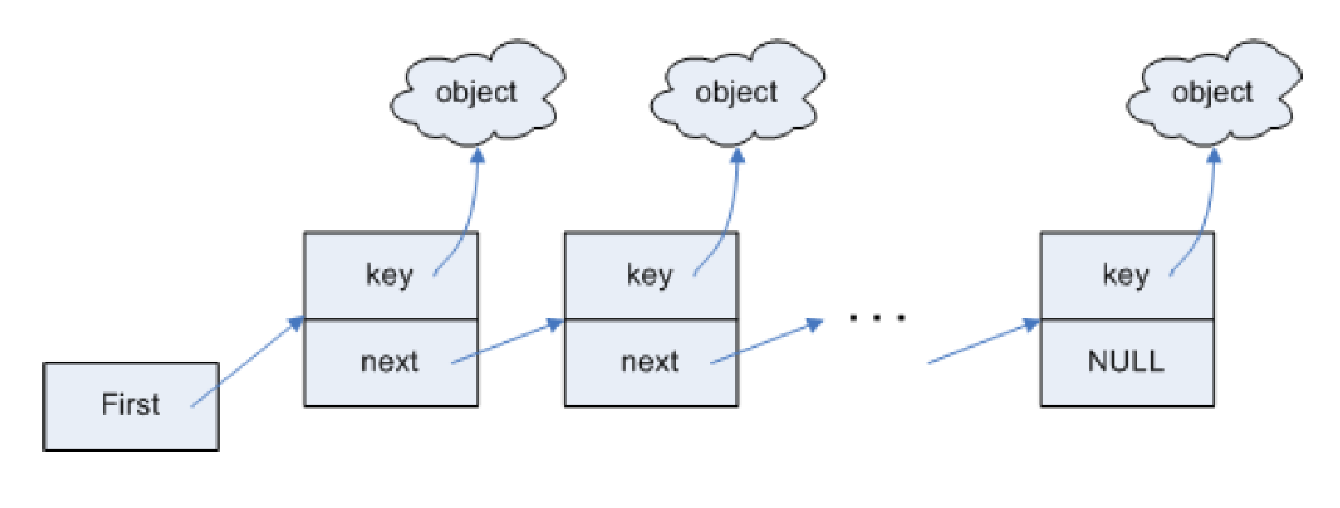
\includegraphics[width=1\linewidth]{1}}
\caption{Структура линейного односвязного списка.}
\end{figure}

\section{Листинг исходного кода}

\lstinputlisting[caption=container.h,language=C++]{./../src/container.h}

\lstinputlisting[caption=container.cpp,language=C++]{./../src/container.cpp}

\lstinputlisting[caption=main.cpp,language=C++]{./../src/main.cpp}


\end{document}